\documentclass[tikz=true]{standalone}
\usepackage{tikz}
\usepackage{../main/NHQM}

\usetikzlibrary{positioning}
%% helper macros

% (fold)
% The 3D code is based on The drawing is based on Tomas M. Trzeciak's 
% `Stereographic and cylindrical map projections example`: 
% http://www.texample.net/tikz/examples/map-projections/
\newcommand\pgfmathsinandcos[3]{%
  \pgfmathsetmacro#1{sin(#3)}%
  \pgfmathsetmacro#2{cos(#3)}%
}
\newcommand\LongitudePlane[3][current plane]{%
  \pgfmathsinandcos\sinEl\cosEl{#2} % elevation
  \pgfmathsinandcos\sint\cost{#3} % azimuth
  \tikzset{#1/.estyle={cm={\cost,\sint*\sinEl,0,\cosEl,(0,0)}}}
}
\newcommand\LatitudePlane[3][current plane]{%
  \pgfmathsinandcos\sinEl\cosEl{#2} % elevation
  \pgfmathsinandcos\sint\cost{#3} % latitude
  \pgfmathsetmacro\yshift{\cosEl*\sint}
  \tikzset{#1/.estyle={cm={\cost,0,0,\cost*\sinEl,(0,\yshift)}}} %
}
\newcommand\DrawLongitudeCircle[2][1]{
  \LongitudePlane{\angEl}{#2}
  \tikzset{current plane/.prefix style={scale=#1}}
   % angle of "visibility"
  \pgfmathsetmacro\angVis{atan(sin(#2)*cos(\angEl)/sin(\angEl))} %
  \draw[current plane,thin,black] (\angVis:1) arc (\angVis:\angVis+180:1);
  \draw[current plane,thin,dashed] (\angVis-180:1) arc (\angVis-180:\angVis:1);
}%this is fake: for drawing the grid
\newcommand\DrawLongitudeCirclered[2][1]{
  \LongitudePlane{\angEl}{#2}
  \tikzset{current plane/.prefix style={scale=#1}}
   % angle of "visibility"
  \pgfmathsetmacro\angVis{atan(sin(#2)*cos(\angEl)/sin(\angEl))} %
  \draw[current plane,red,thick] (150:1) arc (150:180:1);
  %\draw[current plane,dashed] (-50:1) arc (-50:-35:1);
}%for drawing the grid
\newcommand\DLongredd[2][1]{
  \LongitudePlane{\angEl}{#2}
  \tikzset{current plane/.prefix style={scale=#1}}
   % angle of "visibility"
  \pgfmathsetmacro\angVis{atan(sin(#2)*cos(\angEl)/sin(\angEl))} %
  \draw[current plane,black,dashed, ultra thick] (150:1) arc (150:180:1);
}
\newcommand\DLatred[2][1]{
  \LatitudePlane{\angEl}{#2}
  \tikzset{current plane/.prefix style={scale=#1}}
  \pgfmathsetmacro\sinVis{sin(#2)/cos(#2)*sin(\angEl)/cos(\angEl)}
  % angle of "visibility"
  \pgfmathsetmacro\angVis{asin(min(1,max(\sinVis,-1)))}
  \draw[current plane,dashed,black,ultra thick] (-50:1) arc (-50:-35:1);

}
\newcommand\fillred[2][1]{
  \LongitudePlane{\angEl}{#2}
  \tikzset{current plane/.prefix style={scale=#1}}
   % angle of "visibility"
  \pgfmathsetmacro\angVis{atan(sin(#2)*cos(\angEl)/sin(\angEl))} %
  \draw[current plane,red,thin] (\angVis:1) arc (\angVis:\angVis+180:1);

}

\newcommand\DrawLatitudeCircle[2][1]{
  \LatitudePlane{\angEl}{#2}
  \tikzset{current plane/.prefix style={scale=#1}}
  \pgfmathsetmacro\sinVis{sin(#2)/cos(#2)*sin(\angEl)/cos(\angEl)}
  % angle of "visibility"
  \pgfmathsetmacro\angVis{asin(min(1,max(\sinVis,-1)))}
  \draw[current plane,thin,black] (\angVis:1) arc (\angVis:-\angVis-180:1);
  \draw[current plane,thin,dashed] (180-\angVis:1) arc (180-\angVis:\angVis:1);
}%Defining functions to draw limited latitude circles (for the red mesh)
\newcommand\DrawLatitudeCirclered[2][1]{
  \LatitudePlane{\angEl}{#2}
  \tikzset{current plane/.prefix style={scale=#1}}
  \pgfmathsetmacro\sinVis{sin(#2)/cos(#2)*sin(\angEl)/cos(\angEl)}
  % angle of "visibility"
  \pgfmathsetmacro\angVis{asin(min(1,max(\sinVis,-1)))}
  %\draw[current plane,red,thick] (-\angVis-50:1) arc (-\angVis-50:-\angVis-20:1);
\draw[current plane,red,thick] (-50:1) arc (-50:-35:1);

}


\newcommand\DrawOrbitCircle[2][1]{
  \LatitudePlane{\angEl}{#2}
  \tikzset{current plane/.prefix style={scale=#1}}
  \pgfmathsetmacro\sinVis{sin(#2)/cos(#2)*sin(\angEl)/cos(\angEl)}
  % angle of "visibility"
  \pgfmathsetmacro\angVis{asin(min(1,max(\sinVis,-1)))}
  \draw[current plane,thin,gray] (\angVis:1) arc (\angVis:-\angVis-180:1);
  \draw[current plane,thin,gray] (180-\angVis:1) arc (180-\angVis:\angVis:1);
}


\newcommand\DrawArrowOrbitCircle[2][1]{
  \LatitudePlane{\angEl}{#2}
  \tikzset{current plane/.prefix style={scale=#1}}
  \pgfmathsetmacro\sinVis{sin(#2)/cos(#2)*sin(\angEl)/cos(\angEl)}
  % angle of "visibility"
  \pgfmathsetmacro\angVis{asin(min(1,max(\sinVis,-1)))}
  \draw[current plane,thick,gray, mid arrows] (\angVis:1) arc (\angVis:-\angVis-180:1);
  \draw[current plane,thick,gray, mid arrows] (180-\angVis:1) arc (180-\angVis:\angVis:1);
}


\newcommand\proton[1]{%
\shade[ball color=red] (#1) circle(0.5);
}

\newcommand\neutron[1]{%
\shade[ball color=black] (#1) circle(0.5);
}

\newcommand\blobb[1]{%
\shade[ball color=gray] (#1) circle(0.9);
\shade[ball color=red, opacity =0.15] (#1) circle(0.9);
}

% (end)

\tikzset{%
  >=latex,
  inner sep=0pt,%
  outer sep=2pt,%
  mark coordinate/.style={inner sep=0pt,outer sep=0pt,minimum size=3pt,
    fill=black,circle}%
}
\usepackage{amsmath}
\usetikzlibrary{arrows}
\pagestyle{empty}
\usepackage{pgfplots}
\usetikzlibrary{calc,fadings,decorations.pathreplacing}

\begin{document}
  
  %%%%%%%%%%%% He4 DELTA
  
	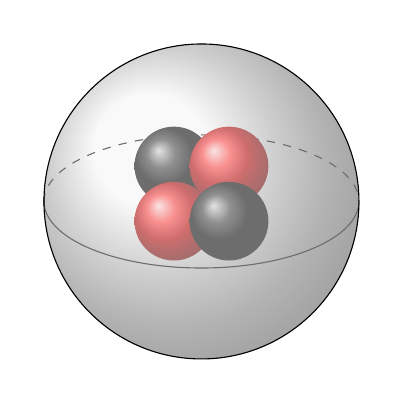
\begin{tikzpicture}[scale=1,every node/.style={minimum size=1cm}]
	%% some definitions
	
	\def\R{2} % sphere radius
	\def\offset{0.1} % sphere radius
	\def\neR{5.25}
	
	\def\angEl{25} % elevation angle
	\def\angAz{-100} % azimuth angle
	\def\angPhiOne{-50} % longitude of point P
	\def\angPhiTwo{-35} % longitude of point Q
	\def\angBeta{30} % latitude of point P and Q
	
	\draw [blue, opacity =0] (-2.2,2.2) rectangle (2.2,-2.2);
	
	%% working planes
	
	\pgfmathsetmacro\H{\R*cos(\angEl)} % distance to north pole
	\LongitudePlane[xzplane]{\angEl}{\angAz}
	\LongitudePlane[pzplane]{\angEl}{\angPhiOne}
	\LongitudePlane[qzplane]{\angEl}{\angPhiTwo}
	\LatitudePlane[equator]{\angEl}{0}
	\fill[ball color=white!5] (0,0) circle (\R); % 3D lighting effect
	\coordinate (O) at (0,0);
	% \coordinate[mark coordinate] (N) at (0,\H);
	% \coordinate[mark coordinate] (S) at (0,-\H);
	\path[xzplane] (\R,0) coordinate (XE);
	
    \DrawLatitudeCircle[\R]{0} % equator
	
	
	\neutron{$(-0.35,\offset + 0.35)$}
	\proton{$(0.35,\offset + 0.35)$}
	\proton{$(-0.35,\offset -0.35)$}
	\neutron{$(0.35,\offset -0.35)$}
	
	\draw[fill = gray!10, fill opacity =0.45, ] (0,0) circle (\R);
	    	
\end{tikzpicture}

%%%%%%%%%%%%%%%% He6 DIM

\usetikzlibrary{fadings}

	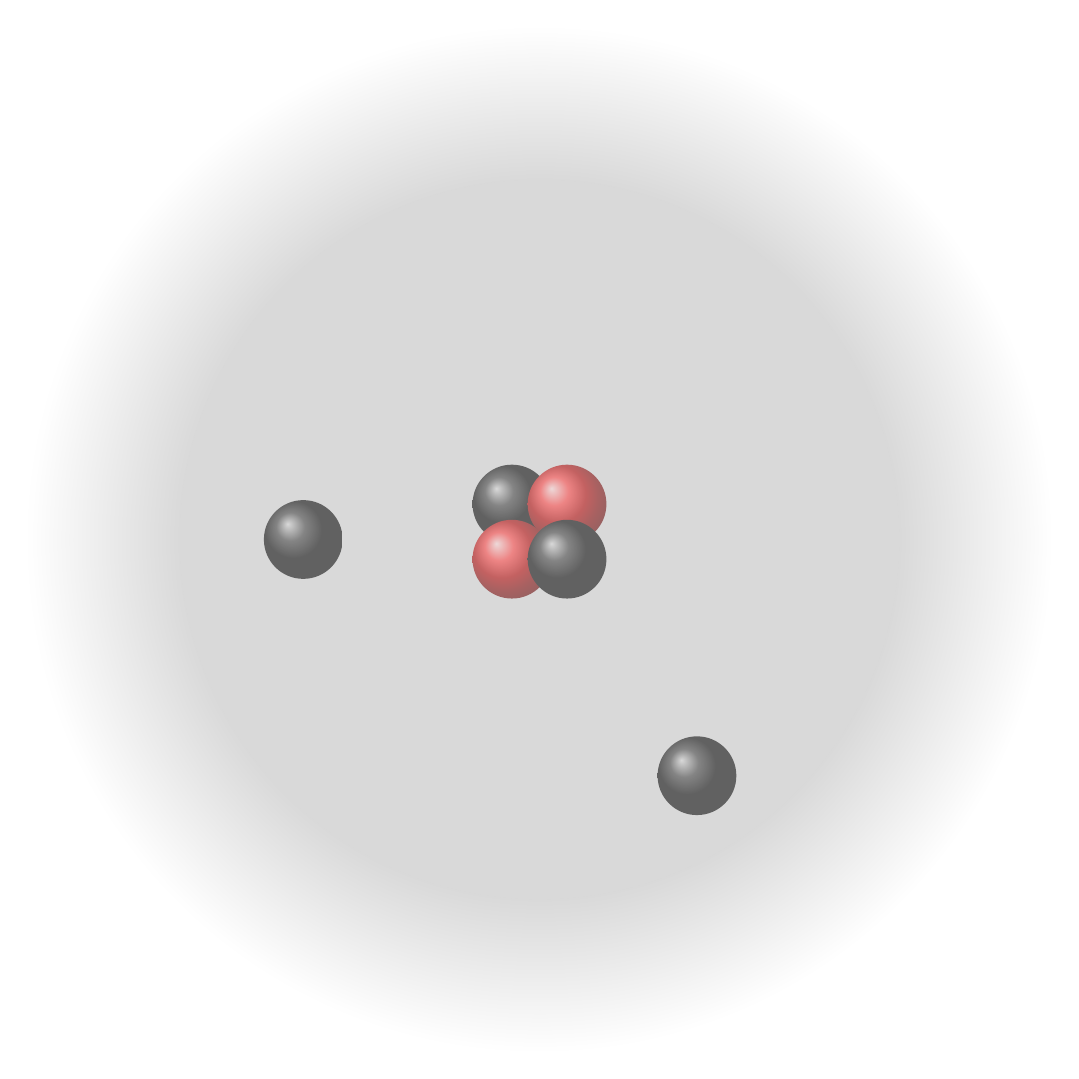
\begin{tikzpicture}[scale=1,every node/.style={minimum size=1cm}]
	%% some definitions
    \tikzfading[name=fade out, inner color=transparent!0, outer color=transparent!100]
	
	
	
	\def\R{2} % sphere radius
	\def\offset{0.1} % sphere radius
	\def\neR{5.25}
	
	
	
		
		
    \fill [gray, path fading=fade out] (0,0) circle (6.5);
	
	\fill [gray!30, fill opacity =1] (0,0) circle (4.57);

%	\fill[ball color=white!5] (0,0) circle (4.57); % 3D lighting effect
	
	% \fill[color = white!5, opacity = 0.7] (-1.5,1.5) circle (1.25);
% 	\fill[color = white!4, opacity = 0.5] (-1.5,1.5) circle (1.55);
% 	\fill[color = white!3, opacity = 0.3] (-1.5,1.5) circle (1.85);
% 	\fill[color = white!2, opacity = 0.1] (-1.5,1.5) circle (2.25);
	
	\def\angEl{25} % elevation angle
	\def\angAz{-100} % azimuth angle
	\def\angPhiOne{-50} % longitude of point P
	\def\angPhiTwo{-35} % longitude of point Q
	\def\angBeta{30} % latitude of point P and Q
	
	
		
	\neutron{$(-0.35,\offset + 0.35)$}
	\proton{$(0.35,\offset + 0.35)$}
	\proton{$(-0.35,\offset -0.35)$}
	\neutron{$(0.35,\offset -0.35)$}

  \neutron{$(-3,0)$}
	\neutron{$(2,-3)$}
	
	\fill[fill = gray!30, fill opacity =0.45, ] (0,0) circle (4.57);
	
	    	
\end{tikzpicture}

%%%%%%%%%%%%%%%% He6 DIM JS

\usetikzlibrary{fadings}

	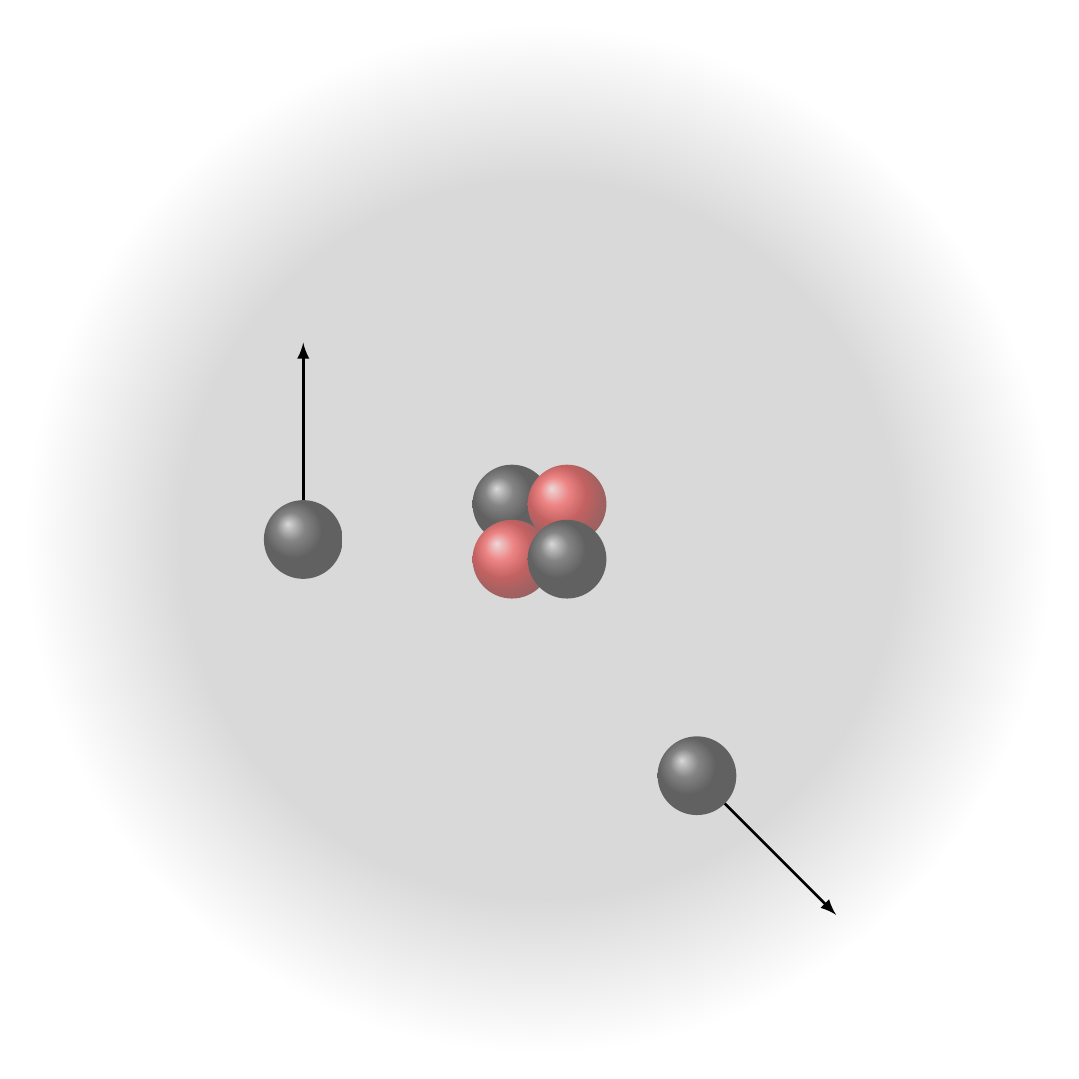
\begin{tikzpicture}[scale=1,every node/.style={minimum size=1cm}]
	%% some definitions
    \tikzfading[name=fade out, inner color=transparent!0, outer color=transparent!100]
	
	
	
	\def\R{2} % sphere radius
	\def\offset{0.1} % sphere radius
	\def\neR{5.25}
	
	
	
		
		
    \fill [gray, path fading=fade out] (0,0) circle (6.5);
	
	\fill [gray!30, fill opacity =1] (0,0) circle (4.57);
  
  
%	\fill[ball color=white!5] (0,0) circle (4.57); % 3D lighting effect
	
	% \fill[color = white!5, opacity = 0.7] (-1.5,1.5) circle (1.25);
% 	\fill[color = white!4, opacity = 0.5] (-1.5,1.5) circle (1.55);
% 	\fill[color = white!3, opacity = 0.3] (-1.5,1.5) circle (1.85);
% 	\fill[color = white!2, opacity = 0.1] (-1.5,1.5) circle (2.25);
	
	\def\angEl{25} % elevation angle
	\def\angAz{-100} % azimuth angle
	\def\angPhiOne{-50} % longitude of point P
	\def\angPhiTwo{-35} % longitude of point Q
	\def\angBeta{30} % latitude of point P and Q
	
	
		
	\neutron{$(-0.35,\offset + 0.35)$}
	\proton{$(0.35,\offset + 0.35)$}
	\proton{$(-0.35,\offset -0.35)$}
	\neutron{$(0.35,\offset -0.35)$}
  
  

  \neutron{$(-3,0)$}
	\neutron{$(2,-3)$}
	
	\fill[fill = gray!30, fill opacity =0.45, ] (0,0) circle (4.57);
  \begin{scope}[->, font=\huge, line width=1pt]
    \draw (-3,0.5) -- ++ (0,2);
    \draw (2,-3) ++ (-45:0.5) -- ++ (-45:2);
  \end{scope}

	    	
\end{tikzpicture}

%%%%%%%%%%%%%%%% He6 DIM TOTAL J

\usetikzlibrary{fadings}

	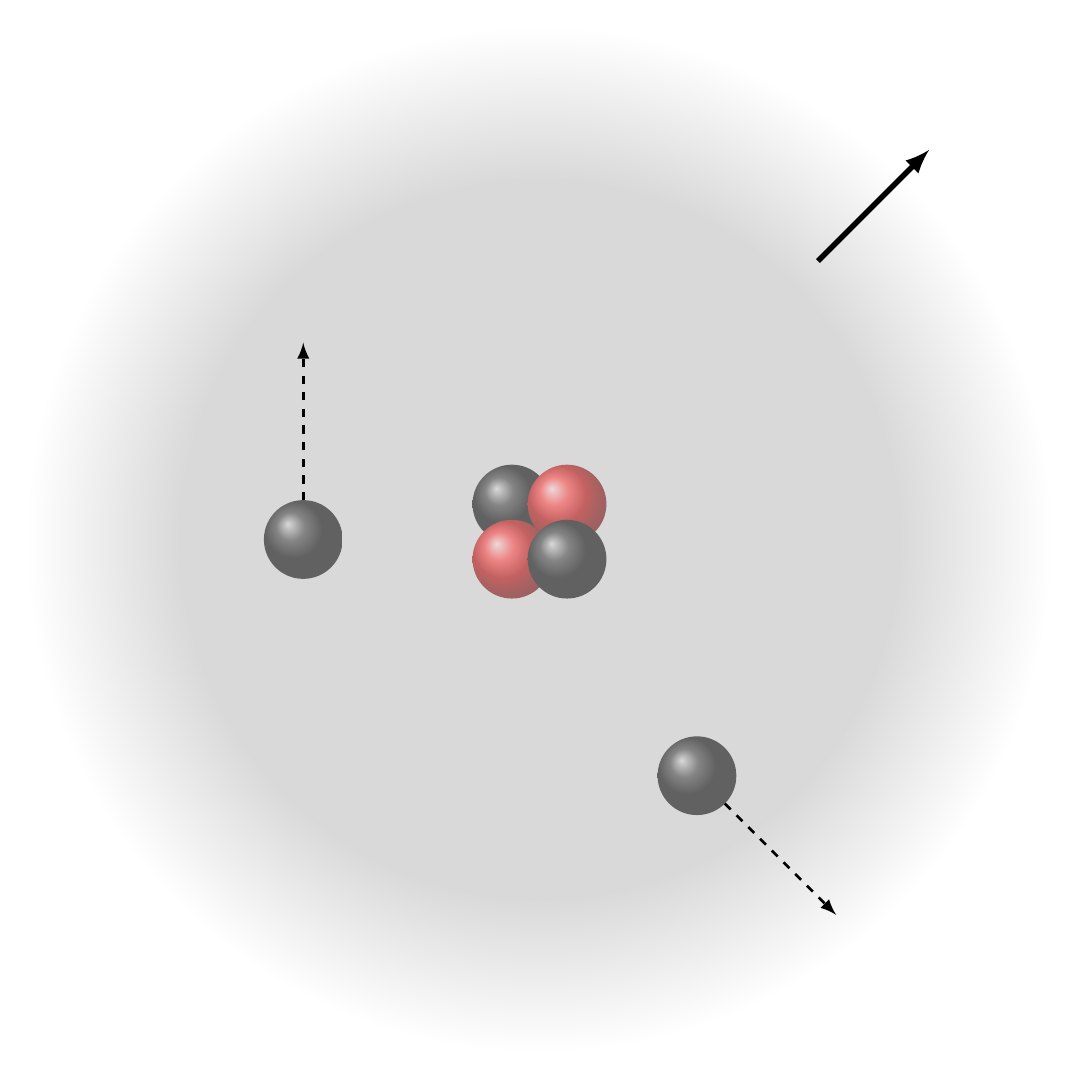
\begin{tikzpicture}[scale=1,every node/.style={minimum size=1cm}]
	%% some definitions
    \tikzfading[name=fade out, inner color=transparent!0, outer color=transparent!100]
	
	
	
	\def\R{2} % sphere radius
	\def\offset{0.1} % sphere radius
	\def\neR{5.25}
	
	
	
		
		
    \fill [gray, path fading=fade out] (0,0) circle (6.5);
	
	\fill [gray!30, fill opacity =1] (0,0) circle (4.57);
  
  
%	\fill[ball color=white!5] (0,0) circle (4.57); % 3D lighting effect
	
	% \fill[color = white!5, opacity = 0.7] (-1.5,1.5) circle (1.25);
% 	\fill[color = white!4, opacity = 0.5] (-1.5,1.5) circle (1.55);
% 	\fill[color = white!3, opacity = 0.3] (-1.5,1.5) circle (1.85);
% 	\fill[color = white!2, opacity = 0.1] (-1.5,1.5) circle (2.25);
	
	\def\angEl{25} % elevation angle
	\def\angAz{-100} % azimuth angle
	\def\angPhiOne{-50} % longitude of point P
	\def\angPhiTwo{-35} % longitude of point Q
	\def\angBeta{30} % latitude of point P and Q
	
	
		
	\neutron{$(-0.35,\offset + 0.35)$}
	\proton{$(0.35,\offset + 0.35)$}
	\proton{$(-0.35,\offset -0.35)$}
	\neutron{$(0.35,\offset -0.35)$}
  
  

  \neutron{$(-3,0)$}
	\neutron{$(2,-3)$}
	
	\fill[fill = gray!30, fill opacity =0.45, ] (0,0) circle (4.57);
  \begin{scope}[->, font=\HUGE, line width=1pt]
    \draw[dashed] (-3,0.5) -- ++ (0,2);
    \draw[dashed] (2,-3) ++ (-45:0.5) -- ++ (-45:2);
    \draw[line width=2pt] (45:5) -- (45:7);
  \end{scope}

	    	
\end{tikzpicture}

%%%%%%%%%%%%%%%% He6 NODIM

\usetikzlibrary{fadings}

	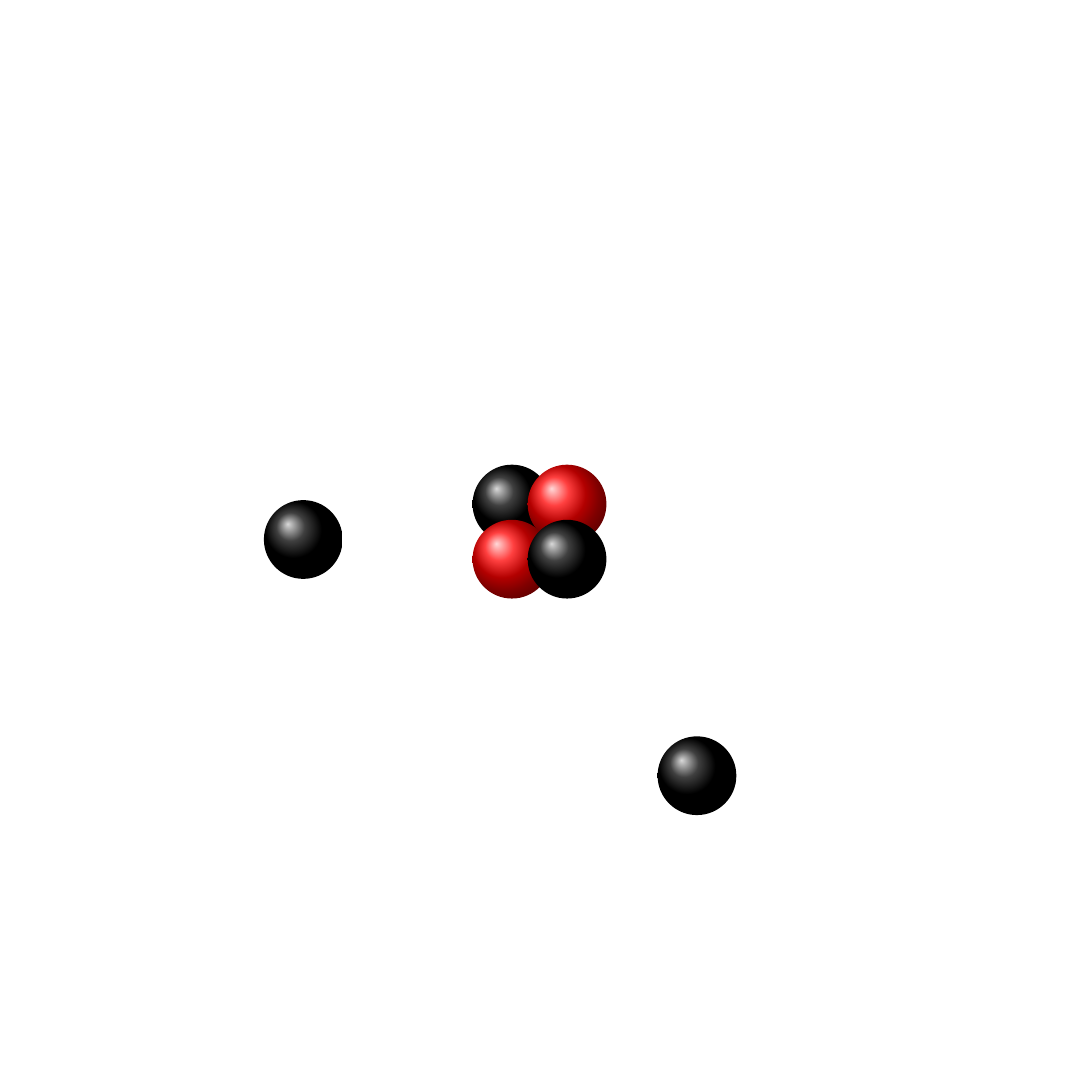
\begin{tikzpicture}[scale=1,every node/.style={minimum size=1cm}]
	%% some definitions
    \tikzfading[name=fade out, inner color=transparent!0, outer color=transparent!100]
	
	
	
	\def\R{2} % sphere radius
	\def\offset{0.1} % sphere radius
	\def\neR{5.25}
	
	
	
		
		
    \clip(0,0) circle (6.5);

%	\fill[ball color=white!5] (0,0) circle (4.57); % 3D lighting effect
	
	% \fill[color = white!5, opacity = 0.7] (-1.5,1.5) circle (1.25);
% 	\fill[color = white!4, opacity = 0.5] (-1.5,1.5) circle (1.55);
% 	\fill[color = white!3, opacity = 0.3] (-1.5,1.5) circle (1.85);
% 	\fill[color = white!2, opacity = 0.1] (-1.5,1.5) circle (2.25);
	
	\def\angEl{25} % elevation angle
	\def\angAz{-100} % azimuth angle
	\def\angPhiOne{-50} % longitude of point P
	\def\angPhiTwo{-35} % longitude of point Q
	\def\angBeta{30} % latitude of point P and Q
	
	
		
	\neutron{$(-0.35,\offset + 0.35)$}
	\proton{$(0.35,\offset + 0.35)$}
	\proton{$(-0.35,\offset -0.35)$}
	\neutron{$(0.35,\offset -0.35)$}

  \neutron{$(-3,0)$}
	\neutron{$(2,-3)$}
	
	    	
\end{tikzpicture}

%%%%%%%%%%%%%%%% He5 He6

\usetikzlibrary{fadings}

	\begin{tikzpicture}[scale=1,every node/.style={minimum size=1cm}]
	%% some definitions
    \tikzfading[name=fade out, inner color=transparent!0, outer color=transparent!100]
	
	
	
	\def\R{2} % sphere radius
	\def\offset{0.1} % sphere radius
	\def\neR{5.25}
	
    \clip (0,0) circle (6.5);

%	\fill[ball color=white!5] (0,0) circle (4.57); % 3D lighting effect
	
	% \fill[color = white!5, opacity = 0.7] (-1.5,1.5) circle (1.25);
% 	\fill[color = white!4, opacity = 0.5] (-1.5,1.5) circle (1.55);
% 	\fill[color = white!3, opacity = 0.3] (-1.5,1.5) circle (1.85);
% 	\fill[color = white!2, opacity = 0.1] (-1.5,1.5) circle (2.25);
	
	\def\angEl{25} % elevation angle
	\def\angAz{-100} % azimuth angle
	\def\angPhiOne{-50} % longitude of point P
	\def\angPhiTwo{-35} % longitude of point Q
	\def\angBeta{30} % latitude of point P and Q
	
	
		
	\neutron{$(-0.35,\offset + 0.35)$}
	\proton{$(0.35,\offset + 0.35)$}
	\proton{$(-0.35,\offset -0.35)$}
	\neutron{$(0.35,\offset -0.35)$}

  \neutron{$(-3,0)$}
	%\neutron{$(2,-3)$}
	
	    	
\end{tikzpicture}

%%%%%%%%%%%%%%%% He6 VXV

\usetikzlibrary{fadings}

	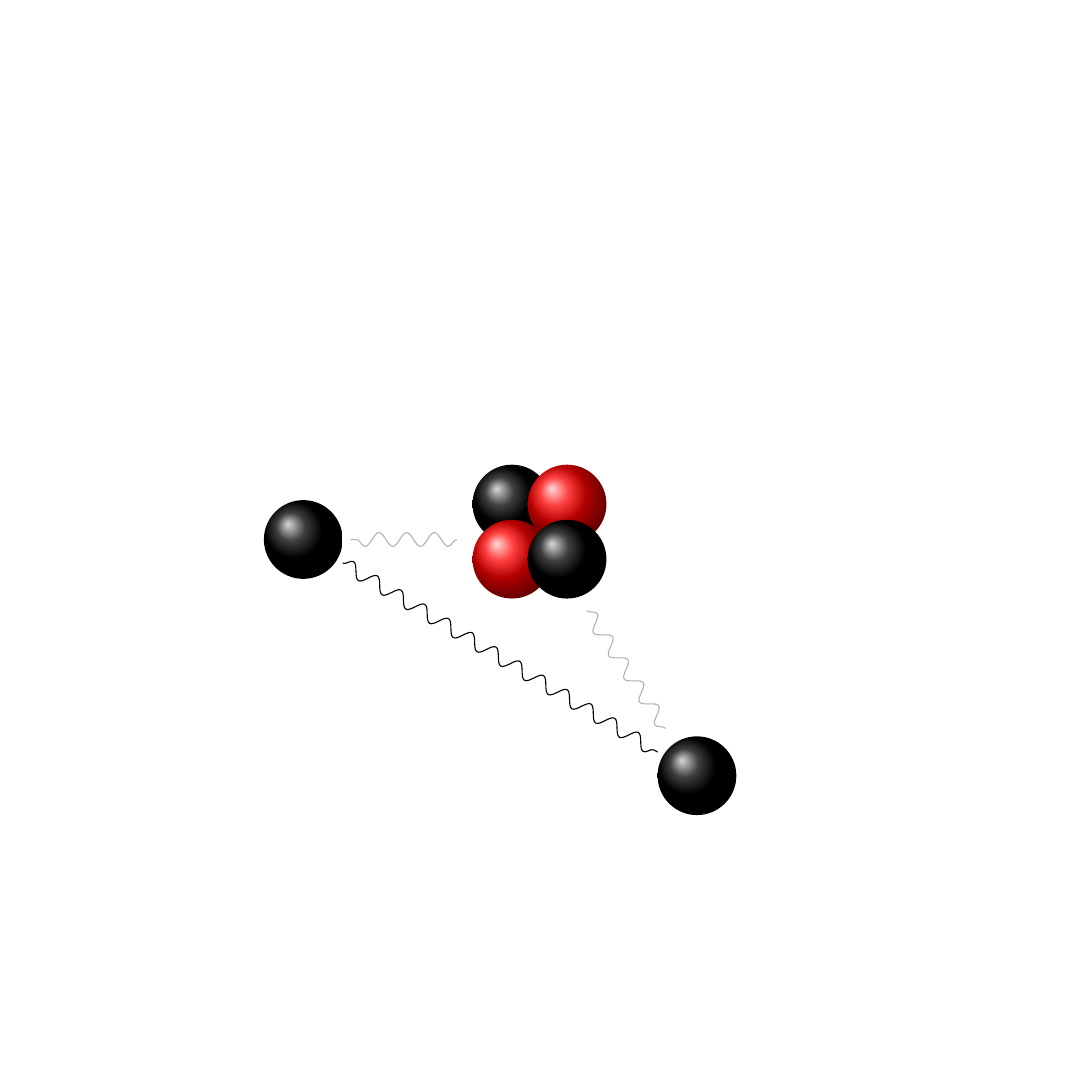
\begin{tikzpicture}[scale=1,every node/.style={minimum size=1cm}]
	%% some definitions
    \tikzfading[name=fade out, inner color=transparent!0, outer color=transparent!100]
	
	
	
	\def\R{2} % sphere radius
	\def\offset{0.1} % sphere radius
	\def\neR{5.25}
	
    \clip (0,0) circle (6.5);

%	\fill[ball color=white!5] (0,0) circle (4.57); % 3D lighting effect
	
	% \fill[color = white!5, opacity = 0.7] (-1.5,1.5) circle (1.25);
% 	\fill[color = white!4, opacity = 0.5] (-1.5,1.5) circle (1.55);
% 	\fill[color = white!3, opacity = 0.3] (-1.5,1.5) circle (1.85);
% 	\fill[color = white!2, opacity = 0.1] (-1.5,1.5) circle (2.25);
	
	\def\angEl{25} % elevation angle
	\def\angAz{-100} % azimuth angle
	\def\angPhiOne{-50} % longitude of point P
	\def\angPhiTwo{-35} % longitude of point Q
	\def\angBeta{30} % latitude of point P and Q
	
	
		
	\neutron{$(-0.35,\offset + 0.35)$}
	\proton{$(0.35,\offset + 0.35)$}
	\proton{$(-0.35,\offset -0.35)$}
	\neutron{$(0.35,\offset -0.35)$}
  \coordinate (a) at (-3,0);
  \coordinate (b) at (2,-3);
  \neutron{$(a)$}
	\neutron{$(b)$}
  \draw[decorate, decoration={snake},]
    ($(a)!0.1!(b)$) -- ($(a)!0.9!(b)$);
  \draw[decorate, decoration={snake},black!30]
    ($(0,0)!0.35!(a)$) -- ($(0,0)!0.8!(a)$);
  \draw[decorate, decoration={snake},black!30]
    ($(0,0)!0.3!(b)$) -- ($(0,0)!0.8!(b)$);
	
	    	
\end{tikzpicture}

%%%%%%%%%%%%%%%%%%%%% He5 LHC

\begin{tikzpicture}
	
	\def\R{2} % sphere radius
	\def\offset{0} % sphere radius

	\def\angEl{25} % elevation angle
	\def\angAz{-100} % azimuth angle
	\def\angPhiOne{-50} % longitude of point P
	\def\angPhiTwo{-35} % longitude of point Q
	\def\angBeta{30} % latitude of point P and Q
	
	\draw [blue, opacity =0] (-3.6,2.5) rectangle (3.2,-2.5);
	
	
	\neutron{$(-0.35,\offset + 0.35)$}
	\proton{$(0.35,\offset + 0.35)$}
	\proton{$(-0.35,\offset -0.35)$}
	\neutron{$(0.35,\offset -0.35)$}


    \DrawArrowOrbitCircle[3]{0} % equator
	
	\draw[thick, mid arrows, gray] (3,-2) -- (-1.25,-1.156);
	\draw[thick, mid arrows, gray] (-1.25,1.156) -- (3,2);

		
	\neutron{$(-3,0)$}
		
\end{tikzpicture}

%%%%%%%%%% He5 BLOBB

 \usetikzlibrary{snakes}
\begin{tikzpicture}
	
	\def\R{2} % sphere radius
	\def\offset{0} % sphere radius

	\def\angEl{25} % elevation angle
	\def\angAz{-100} % azimuth angle
	\def\angPhiOne{-50} % longitude of point P
	\def\angPhiTwo{-35} % longitude of point Q
	\def\angBeta{30} % latitude of point P and Q
	
	
	\draw [blue, opacity =0] (-3.6,2.5) rectangle (3.2,-2.5);
	
	\blobb{0,0}
	\begin{scope}[, decoration={snake, post length=0}, gray]
		 \draw[decorate] (-2.4,0) -- (-1.05,0);
	\end{scope}
	
	\begin{scope}[opacity=0.1]
    \DrawArrowOrbitCircle[3]{0} % equator
	
  	\draw[thick, mid arrows, gray] (3,-2) -- (-1.25,-1.156);
  	\draw[thick, mid arrows, gray] (-1.25,1.156) -- (3,2);
	\end{scope}


	
	\neutron{$(-3,0)$}
		
\end{tikzpicture}

%%%%%%%%%%%%%%%%%%%%%%%%%%%%%%%%%%%%%%%%%%%%%%%%%%%%%%%%%%%%%%%%%%%%55

    \begin{tikzpicture}
      \begin{axis}[
        font=\Large,
        xlabel = $r_1$,
        ylabel = V,
        axis x line = middle,
        axis y line = left,
        xtick=\empty,
        ytick={0},
        yticklabels={0},
        domain=0:3,
        ymin=-1.2, ymax=0.5,
        every axis y label/.style={
          at = {(current axis.above origin)},
          anchor = north west,
        },
		after end axis/.code={
		               \draw[anchor=west, dashed] (axis cs:0,-1) -- (axis cs:1,-1) 
					   node [font=\Large] {$\displaystyle -V_0\exp\p{-\frac{r_2^2}{R^2}}$};
		             },
        ]
        \addplot[thick, black] {-e^(-x^2)};		
      \end{axis}
    \end{tikzpicture}
%%%%%%%%%%%%%%%%%%%%%%%%%%%%%%%%%%%%%%%%%%%%%%%%%%%%%%%%%%%%%%%%%%

  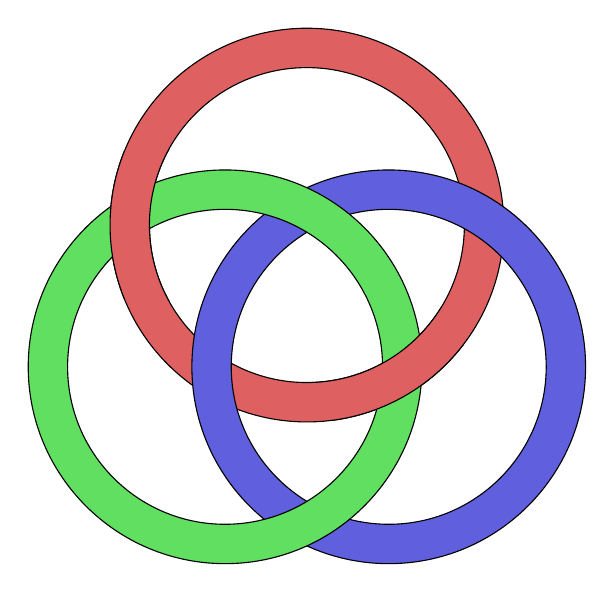
\begin{tikzpicture}[even odd rule]
  	\newcommand{\circdist}{1.2}
	\newcommand{\circrad}{2}
    \foreach \angle/\colour in {90/red!50!lightgray,-30/blue!50!lightgray,210/green!50!lightgray}
      \draw [fill=\colour] 
        (\angle:\circdist) circle (\circrad) circle (\circrad+0.5);

    \begin{scope}
    \clip (-30:\circdist) circle (1);
    \draw [fill=red!50!lightgray] (90:\circdist) circle (\circrad) circle (\circrad+0.5);
    \end{scope}

    \clip (90:\circdist) ++ (180:\circrad) circle (1);
    \draw [fill=red!50!lightgray] (90:\circdist) circle (\circrad) circle (\circrad+0.5);
  \end{tikzpicture}

\end{document} 
